\chapter{Gait generation via IS-MPC}
\section{Gait generation via IS-MPC (from WoS)}
\label{sec:WoS:offlineCase:GaitGeneration}
The gait generation module receives the planned footstep sequence ${\cal S}_f$ as input, and it is in charge of producing a CoM trajectory that the robot can safely track in order to step over said footstep sequence. Along the entire motion, dynamic balance must be maintained.

On flat ground, it is common to ensure dynamic balance as a geometric criterion, by requiring that the ZMP must always be inside the convex hull of contact surfaces, i.e., the \emph{support polygon}. Traditionally, the ZMP is assumed to be located on the ground plane, which is uniquely defined when the environment is flat.

In non-flat environments, there is no unique ground surface on which the ZMP can be assumed to be. However, the aforementioned criterion can be extended to these cases by allowing the ZMP to move in 3D \cite{SuImYaCa:2021}. The balance criterion is satisfied as long as the ZMP is inside a three-dimensional \emph{support region} $\mathcal{Z}$ that takes the shape of a pyramid (see Fig.~\ref{fig:WoS:balance3d}). The vertex of this pyramid is the robot CoM, and the edges are the lines connecting the CoM to the vertexes of the convex hull of the contact surfaces.

In MPC, dynamic balance is enforced via constraints on the ZMP position. However, the 3D support region $\mathcal{Z}$ cannot be directly employed to enforce a ZMP constraint, because this would be nonlinear, meaning that the resulting optimization problem would not be in a standard linear-quadratic formulation. The cause of this nonlinearity is given by the fact that the vertex of the pyramid $\mathcal{Z}$ is the CoM. Since both the ZMP and the CoM depend on the decision variables of the QP, this would result in product between the decision variables themselves.

In order to avoid this, we will define a smaller region, independent of the CoM position, where the ZMP is allowed to be. Furthermore, we will prove that this region conservatively approximates the actual support region $\mathcal{Z}$, and thus that the balance condition is always satisfied under the imposed constraints.

In this section we will describe the MPC gait generation scheme that is used in the proposed formulation. In particular, we will derive the prediction model and define the constraints that ensure stability and dynamic balance. Finally, we will state the QP problem to be solved at each iteration, and give a sketch of the complete algorithm.

\smallskip

\subsection{Prediction Model}

Control of the ZMP is achieved using a dynamic model relating the position of the latter to the position and acceleration of the CoM. This dynamic model can be derived by balancing moments on the humanoid as a whole, and assuming that the rate of change of angular momentum around the CoM can be neglected. With this in mind, denoting the CoM as $\bfp_c = (x_c, y_c, z_c)$ and the ZMP as $\bfp_z = (x_z, y_z, z_z)$, we get
\begin{equation}\begin{split}
(z_c - z_z)\ddot x_c &= (x_c - x_z)(\ddot z_c - g) \\
(z_c - z_z)\ddot y_c &= (y_c - y_z)(\ddot z_c - g),
\end{split}\end{equation}
where $g$ is the gravity acceleration.

This model exhibits a nonlinear coupling between the vertical and the horizontal components of $\bfp_c$ and $\ddot\bfp_c$. On flat ground, this nonlinearity is usually handled by assuming a constant CoM height, which leads to the well-known LIP model~\cite{KaKaKaFuHaYoHi:03}. In order to allow for vertical movement of the CoM, a different choice is made here, which is to constrain the motion of the CoM to satisfy the relation $(\ddot z_c - g)/(z_c - z_z) = \eta^2$, where $\eta$ is a constant parameter.
The resulting dynamic model can be expressed in the form
\begin{equation}\label{eq:WoS:3dmodel}
\ddot \bfp_c = \eta^2(\bfp_c - \bfp_z) - \bfg,
\end{equation}
where $\bfg = (0\,\,\,0\,\,\,g)^T$ is the gravity acceleration vector. This model features a LIP-like dynamic behavior along all three axes. The only difference with respect to a standard LIP is given by the gravity vector $\bfg$ acting as a constant drift. This causes the system not to be in equilibrium when the CoM and ZMP coincide, but rather when they are displaced by $\bfg/\eta^2$.

The choice of restricting the available trajectories to those resulting in a constant $\eta$ allows to make the prediction model linear. If this restriction is removed, the model is referred to as Variable-Height Inverted Pendulum, which can be treated either as nonlinear or time-varying. This can allow for more general motions to be generated, e.g., running~\cite{Smaldone2022Running}, at the cost of a slightly more complex architecture. For the present case, where only walking is considered, the simpler model is preferred.

In order to obtain smoother trajectories, model (\ref{eq:WoS:3dmodel}) is dynamically extended to have the derivative of the ZMP $\dot \bfp_z$ as the input.
The gait generation scheme works over discrete time-steps of duration $\delta$, over which the input $\dot \bfp_z$ is assumed to be constant, i.e., $\dot \bfp_z(t) = \dot \bfp_z^k$ for $t\in[t_k, t_{k+1})$.
This prediction model is used to forecast the evolution of the system over a receding horizon window called the \emph{control horizon}, spanning a time $T_c=C\delta$. The number of steps that are contained, either fully or partially, within this control horizon is denoted as $F$.

\smallskip

\subsection{Stability Constraint}

Model~(\ref{eq:WoS:3dmodel}) has a positive eigenvalue $\eta$, reflecting the intrinsic instability of the humanoid dynamics. Given this instability, it is not sufficient to generate a gait such that the ZMP is inside the support region, because the associated CoM trajectory might be divergent, making the motion unrealizable by the humanoid.
The role of the stability constraint is to enforce a condition on the unstable component of the dynamics in order to guarantee that the CoM trajectory does not diverge with respect to the ZMP.

The unstable component of system (\ref{eq:WoS:3dmodel}) is highlighted by the coordinate $\bfp_u = \bfp_c + \dot \bfp_c/\eta$,
also referred to as Divergent Component of Motion (DCM) or Capture Point (CP), that evolves according to the dynamics
\begin{equation}
\dot\bfp_u = \eta(\bfp_u - \bfp_z) - \frac{\bfg}{\eta}.
\end{equation}
Despite the instability, the evolution of the system is bounded if the following \emph{stability condition} is satisfied
\begin{equation}
\label{eq:WoS:stabilitycondition}
\bfp_u^k = \eta\int_{t_k}^{\infty}e^{-\eta(\tau - t_k)}\bfp_z(\tau) d\tau + \frac{\bfg}{\eta^2},
\end{equation}
as stated by the following proposition.

\medskip

\begin{proposition}
Consider system~(\ref{eq:WoS:3dmodel}). If the ZMP velocity is bounded, 
$|\dot x_z|\le v^{\rm max}$, $|\dot y_z|\le v^{\rm max}$, $|\dot z_z|\le v^{\rm max}$, for some $v^{\rm max}>0$, and condition~(\ref{eq:WoS:stabilitycondition}) is satisfied, then the following bound holds:
\begin{equation}
\label{eq:WoS:ZMPbound}
\frac{\bfg}{\eta^2}- \frac{v^{\rm max}}{\eta}{\bf 1} \le \bfp_c-\bfp_z \le \frac{\bfg}{\eta^2}+\frac{v^{\rm max}}{\eta}{\bf 1},
\end{equation}
where ${\bf 1}$ is a vector with all components equal to 1. Moreover, (\ref{eq:WoS:ZMPbound}) implies that the system is internally stable, i.e., the CoM is bounded with respect to the ZMP.
\label{prop:velocityBound}
\end{proposition}

\medskip

\emph{Proof}. See Appendix.

\medskip

Condition~(\ref{eq:WoS:stabilitycondition}) is non-causal as it requires knowledge of the future ZMP trajectory $\bfp_z$ up to infinity. In order to derive a causal implementation, we split the integral at $t_{k+C}$. Of the two separate integrals that result, the first, over $[t_k, t_{k+C})$, can be expressed in terms of the MPC decision variables. A value for the second integral, over $[t_{k+C}, \infty)$, can be obtained by conjecturing a ZMP trajectory using information coming from the footstep plan.
This conjectured trajectory is called \emph{anticipative tail} and is denoted with $\tilde \bfx_z$. 
In \cite{ScDeLaOr:20}, the anticipative tail was used to prove recursive feasibility and stability of the MPC scheme.

The stability constraint is then written as
\begin{equation}\label{eq:WoS:stability_constraint}
\eta\int_{t_k}^{t_{k+C}}e^{-\eta(\tau - t_k)}\bfp_z d\tau = \bfp_u^k - \tilde \bfc^k - \frac{\bfg}{\eta^2}.
\end{equation}
where $\tilde \bfc^k$ is given by
\begin{equation}%\label{eq:WoS:stability_constraint}
\tilde\bfc^k = \eta\int_{t_{k+C}}^{\infty}e^{-\eta(\tau - t_k)}\tilde\bfp_z d\tau.
\end{equation}

Note that in \cite{ScDeLaOr:20} we considered the footstep plan to be available over a receding window called the \emph{preview horizon}. Here there is no need to make such an assumption, as the footstep plan is provided in its entirety, and once the goal is reached the robot comes to a complete stop.

Enforcing constraint (\ref{eq:WoS:stability_constraint}) allows, similarly to what stated in Prop.~\ref{prop:velocityBound}, to bound the displacement between CoM and ZMP. In fact, the value of the bound is almost identical in most practical situation, especially in view of the fact that the preview horizon is unlimited because the plan is completely known. Because of this fact, we will assume in the following that Prop.~\ref{prop:velocityBound} is valid as stated, even though a small numerical correction should be applied to make up for the difference between the stability condition and the stability constraint.



\smallskip

\subsection{ZMP Velocity Constraint}

This constraint imposes a limit on how fast the ZMP can move, i.e.,
\begin{equation}\label{eq:WoS:ZMP_velocity_constraint}
|\dot x_z|\le v^{\rm max}, \quad |\dot y_z|\le v^{\rm max}, \quad |\dot z_z|\le v^{\rm max}
\end{equation}
Enforcing such limit allows to indirectly control the maximum CoM/ZMP displacement, by using the result of Prop.~\ref{prop:velocityBound}. This will be useful when defining the ZMP position constraint, as will be made clear in the following paragraphs.

\smallskip

\subsection{ZMP Position Constraint}
As already noted, the humanoid is balanced as long as the ZMP is inside the pyramid $\cal Z$, which is a nonlinear condition due to the vertex of the pyramid being at the CoM (Fig. \ref{fig:WoS:balance3d}). To preserve linearity we consider a smaller allowed region for the ZMP, consisting in a box of fixed size with changing center and orientation. We refer to this as the {\em moving box}\footnote{Approximating the pyramidal region $\cal Z$ with a box might seem overly conservative. However, we argue that the neglected portion of the pyramid region is not crucial here, because large displacements of the ZMP in the $z$ direction would only be required to generate large vertical accelerations, which are not necessary in the considered setting (walking in a world of stairs). Clearly, less conservative approximations can still be envisaged and used for generating more dynamic motions.}, and we will prove that it conservatively approximates the support region, meaning that it is always contained inside the pyramid $\cal Z$.



%However, we argue that the neglected portion of the pyramid region is not crucial here, because large displacements of the ZMP in the $z$ direction are only required to generate large vertical accelerations, which are not necessary in the considered setting (walking in a world of stairs).



\begin{figure}
    \centering
    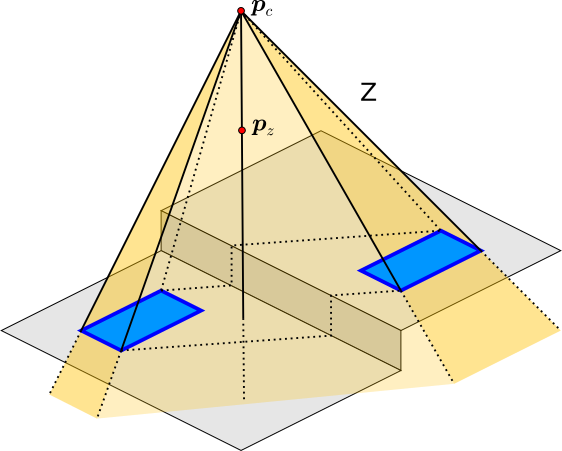
\includegraphics[width=0.6\textwidth]{figures/balance3d.pdf}
    \caption{Balance condition in 3D: the ZMP must lie inside the yellow pyramid.}
    \label{fig:WoS:balance3d}
\end{figure}

\begin{figure}
    \centering
    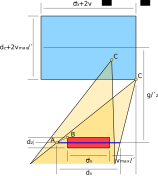
\includegraphics[width=0.6\textwidth]{figures/conservative.pdf}
    \caption{The red rectangle represents a section of the moving box in the $x$-$z$ plane. This region is fully contained inside the yellow pyramid as long as the CoM belongs to the blue region. Here, two scenarios are considered: one in which the CoM is well within the blue region, and a worst-case scenario in which the CoM is in a lower vertex of the blue region.}
    \label{fig:WoS:conservative}
\end{figure}

The center $\bfp_{\rm mc}$ and orientation $\theta_{\rm mc}$ of the moving box are taken to be consistent with the pose of footstep $\bff^j$ during the $j$-th single support phase. In the following double support phase they will gradually slide in order to reach the pose of the next footstep $\bff^{j+1}$, with a linear\footnote{The timing law can be arbitrarily chosen as long as it leads the moving box from one footstep to the next within the duration of the double support phase.} timing law. At each time $t$, the center of the moving box $\bfp_{\rm mc}$ is expressed as
\begin{equation}\label{eq:WoS: moving constraint}
\bfp_{\rm mc}(t) = \Bigg\{
\begin{array}{ll}
\bfp^j & t\in [t_s^j, t_s^j + T_{\rm ss}^j) \\
(1-\alpha^j(t))\bfp^j + \alpha^j(t)\bfp^{j+1} & t\in [t_s^j + T_{\rm ss}^j, t_s^{k+1})
\end{array}
\end{equation}
where $j=0,\dots,F$ is a index over the footsteps within the control horizon, and $\alpha^j(t) = (t-t_s^j-T_{\rm ss}^j)/T_{\rm ds}^j$ denotes the time elapsed since the start of the double support phase, expressed as a fraction of the duration of the double support phase itself.
The orientation of the moving box $\theta_{\rm mc}$ can be similarly expressed as
\begin{equation}\label{eq:WoS: moving constraint angle}
\theta_{\rm mc}(t) = \Bigg\{
\begin{array}{ll}
\theta^j & t\in [t_s^j, t_s^j + T_{\rm ss}^j) \\
\mathrm{anglin}(\theta^j,\theta^{j+1},\alpha^j(t)) & t\in [t_s^j + T_{\rm ss}^j, t_s^{k+1})
\end{array}
\end{equation}
where $j=0,\dots,F$, and $\mathrm{anglin}$ is a function\footnote{For two generic angles
$\theta_a$ and $\theta_b$, linearly combined with a weight $\alpha$, the function $\mathrm{anglin}$ can be defined as
\begin{equation*}\begin{split}
\mathrm{anglin}(\theta_a, \theta_b, \alpha) = \mathrm{atan2}(&\sin((1-\alpha)\theta_a) + \sin(\alpha\theta_b), \\&\cos((1-\alpha)\theta_a) + \cos(\alpha\theta_b)).
\end{split}\end{equation*}
Note that this definition is meaningless when the two angles are separated by exactly $\pi$, but this can never occur as the angle between consecutive footsteps is limited by requirement R2. } that computes a linear combination of angles in such a way to correctly account for wrapping around $\pm\pi$.

The ZMP position constraint is expressed as
\begin{equation}\label{eq:WoS:ZMP_constraint}
-\tilde\bfd /2 \le \bfR_{k+i}^T(\bfp_z^{k+i} - \bfp_{\rm mc}^{k+i}) \le \tilde\bfd /2
\end{equation}
where $\bfp_z^{k+i}$ and $\bfp_{\rm mc}^{k+i}$ respectively denote the ZMP and the center of the moving box sampled at time $t_{k+i}$, $\tilde \bfd = (\tilde d_x, \tilde d_y, d_z)^T$
is a vector collecting the dimensions of the moving box along all three axes, and $\bfR_{k+i}$ is the rotation matrix associated with $\theta_{\rm mc}^{k+i}$.

The size of the moving box $\tilde \bfd = (\tilde d_x, \tilde d_y, d_z)^T$ is determined in such a way to always be contained inside the pyramid $\cal Z$, as expressed by the following proposition.

\medskip

\begin{proposition}
Assume the stability constraint~(\ref{eq:WoS:stability_constraint}) and the ZMP velocity constraint~(\ref{eq:WoS:ZMP_velocity_constraint}) are enforced. If $v^{\rm max}$ is chosen in such a way that
\begin{equation}
v^{\rm max} \le \min \{v_y^{\rm max},v_x^{\rm max}\},
\end{equation}
where $v_x^{\rm max}$ and $v_y^{\rm max}$ are given by the following compact expression
\begin{equation}\label{eq:WoS:conservative_condition}
v_{x,y}^{\rm max} = \eta\left(g/\eta^2 - d_{x,y}\frac{d_z}{d_{x,y} - \tilde d_{x,y}}\right)\left(1 + \frac{d_z}{d_{x,y} - \tilde d_{x,y}}\right)^{-1},
\end{equation}
with $d_x$ and $d_y$ denoting the size of the actual footprint, then the moving box is always contained in the pyramid $\cal Z$.
\label{prop:conservative-box}
\end{proposition}

\medskip

{\em Proof}: Consider the geometric construction in Fig.~\ref{fig:WoS:conservative}. This construction shows a projection of the pyramid ${\cal Z}$ in the $x$-$z$ plane during a single support phase. The red area represents a cross section of the moving box, with dimensions $\tilde d_x$ and $d_z$. The blue area represents the region where the CoM can be found, given the CoM/ZMP bounds~(\ref{eq:WoS:ZMPbound}). In the figure two different possibilities are depicted for the CoM position (identified by the point $C$). Among them, consider the worst-case scenario, in which the CoM is in the bottom-right corner of the blue region\footnote{An equivalent symmetrical scenario would occur if the CoM were in the bottom-left corner. }. A condition for which the red region is always fully contained inside $\cal Z$ can be found by imposing that the slope of the segment $AB$ is less than the slope of the segment $AC$, i.e.,
\begin{equation}
\frac{d_z/2}{d_x/2 - \tilde d_x/2} \le \frac{g/\eta^2 - d_z/2 - v^{\rm max}_x/\eta}{d_x/2 + \tilde d_x/2 + v^{\rm max}_x/\eta},
\end{equation}
which, after simple manipulations, leads to (\ref{eq:WoS:conservative_condition}). During double support phases the construction of Fig.~\ref{fig:WoS:conservative} is not accurate anymore, as the pyramid $\mathcal{Z}$ is much larger than the one represented. However, it is not necessary to repeat the reasoning, as a smaller pyramid, analogous to that shown in Fig.~\ref{fig:WoS:conservative}, can always be constructed and will always be contained inside $\mathcal{Z}$. The last step is to repeat the construction in the $y$-$z$ plane in order to find $v_y^{\rm max}$, which proves the thesis.
\hfill\bull
\smallskip
\subsection{QP Problem}
At a generic time $t_k$, IS-MPC solves the following QP problem

\smallskip

\begin{braced}
\[
\min_{\dot \bfp_z^k, \dots, \dot \bfp_z^{k+C-1}} \quad \sum_{i=0}^{C-1} \left(\|\dot\bfp_z^{k+i}\|^2 + \beta\|\bfp_z^{k+i} - \bfp_{\rm mc}^{k+i}\|^2\right)
\]
\hspace{0.25cm} subject to:
\begin{itemize}
\item stability constraint (\ref{eq:WoS:stability_constraint})
\item ZMP velocity constraint (\ref{eq:WoS:ZMP_velocity_constraint})
\item ZMP position constraint (\ref{eq:WoS:ZMP_constraint})
\end{itemize}
\end{braced}
\smallskip
The cost function minimizes the decision variables (ZMP derivative) as a regularization term, and attempts to bring the ZMP close to the center of the moving box, which is typically beneficial as it produces a more robust walking pattern. $\beta$ is a weight on the second term.

In typical MPC fashion, the first sample of the ZMP velocity $\dot \bfp_z^k$ is used to integrate the 3D LIP dynamics (\ref{eq:WoS:3dmodel}). The resulting CoM trajectory $\bfp_c$ is sent, together with the swing foot trajectory generated by the footstep planner and sampled at time $t_k$, to the kinematic controller.

\subsection{Proof of Prop. \ref{prop:velocityBound}}
\label{sec:WoS:Proof}

Starting from the initial condition $\bfp_u(t_k)$ described by (\ref{eq:WoS:stabilitycondition}), the unstable coordinate $\bfp_u$ evolves as
\begin{equation}
\label{eq:WoS:bounded_evolution}
\bfp_u(t) = \eta\int_{t}^\infty e^{-\eta(\tau-t)}\bfp_z(\tau) d\tau + \frac{\bfg}{\eta^2}.
\end{equation}
Integrating \ref{eq:WoS:bounded_evolution} by parts gives
\begin{equation}
\label{eq:WoS:bounded_evolution_integrated}
\bfp_u(t) - \bfp_z(t) - \frac{\bfg}{\eta^2} = \int_{t}^\infty e^{-\eta(\tau-t)}\dot\bfp_z d\tau.
\end{equation}
Since by hypothesis the ZMP velocity $\dot\bfp_z$ is component-wise bounded, i.e., $|\dot x_z| \le v^{\rm max}$, $|\dot y_z| \le v^{\rm max}$, $|\dot z_z| \le v^{\rm max}$, then the following upper bound is obtained
\begin{equation*}
\bfp_u(t) - \bfp_z(t) - \frac{\bfg}{\eta^2} \leq v^{\rm max}{\bf 1}\int_{t}^\infty e^{-\eta(\tau-t)}  d\tau,
\end{equation*}
along with a similar lower bound.
%Since the ZMP velocity constraint is enforced, the components of $\dot\bfp_z$ are bounded by $|\dot x_z| \le v_{\rm max}$, $|\dot y_z| \le v_{\rm max}$, $|\dot z_z| \le v_{\rm max}$. Thus, by evaluating the integral, we obtain
The two bounds can be combined in the following expression
\begin{equation}
\label{eq:WoS:bound unstable}
-\frac{v^{\rm max}}{\eta}{\bf 1}
\le
\bfp_u(t) - \bfp_z(t) - \frac{\bfg}{\eta^2}
\le
\frac{v^{\rm max}}{\eta}{\bf 1}.
\end{equation}

Define now the coordinate $\bfp_s = \bfp_c - \dot \bfp_c/\eta$. This coordinate pertains to the stable eigenvalue of system (\ref{eq:WoS:3dmodel}), and its dynamics can be expressed as
\begin{equation*}
\dot\bfp_s = \eta(-\bfp_s + \bfp_z) + \frac{\bfg}{\eta}.
\end{equation*}
Starting from an initial time $t_0$, the coordinate $\bfp_s$ evolves as
\begin{equation*}
\bfp_s(t) = \bfp_s(t_0) e^{-\eta(t-t_0)} + \eta\int_{t_0}^t e^{-\eta(t-\tau)}\left(\bfp_z(\tau)  +\frac{\bfg}{\eta^2}\right)d\tau.
\end{equation*}
Similarly to $\bfp_u$, the above expression can manipulated using integration by parts, and the resulting integral can be bounded using the hypothesis on the ZMP velocity. The resulting expression is
\begin{equation*}
-\frac{v^{\rm max}}{\eta}{\bf 1} + \bfs_0
\le
\bfp_s(t) - \bfp_z(t) - \frac{\bfg}{\eta^2}
\le
\frac{v^{\rm max}}{\eta}{\bf 1} + \bfs_0,
\end{equation*}
where $\bfs_0 = \bfp_s(t_0) - \bfp_z(t_0) - \bfg/\eta^2$. 
Since at $t_0$ the robot is typically in static equilibrium, corresponding to $\bfp_c(t_0) = \bfp_z(t_0) + \bfg/\eta^2$ and $\dot{\bfp}_c(t_0) = 0$, then $\bfs_0 = 0$. This leads to
\begin{equation}
-\frac{v^{\rm max}}{\eta}{\bf 1}\label{eq:WoS:bound stable}
\le
\bfp_s(t) - \bfp_z(t) - \frac{\bfg}{\eta^2}
\le
\frac{v^{\rm max}}{\eta}{\bf 1}.
\end{equation}
By noting that $2\bfp_c = \bfp_u + \bfp_s$, combining eqs. (\ref{eq:WoS:bound unstable}) and (\ref{eq:WoS:bound stable}) proves the thesis.
